%!TEX root = ../dissertation.tex

\chapter{Introduction}
\label{chapter:introduction}

%Motivation
%Goals
%Thesis Outline

\section{From Paper to Bits}
%(paper)
%(drafting: sketchpad, cad mainframes, autocad2d)
%(3d)
%(2d + 3d + analysis + visualization)

Through the years, computers have been taking more ground in the field of architecture.
It began with the appearance of Sketchpad\cite{Sutherland:1964:SPM:800265.810742} in the 60s that showed that computers could be used to create drawings interactively.
After the appearance of desktop computers, drafting software like AutoCAD popularized \gls{cad} in architecture.
As opposed to drawing by hand, using computers to create these drawings allowed architects to make changes without having to redraw the drawings, therefore saving them much time.
Still, computers were only used for creating technical drawings, leaving most of the thinking about 3D space outside of the computer.

As computers became powerful enough to display 3D graphics, and 3D modeling started to appear, it became possible to model buildings in the computer and preview them in interactive 3D views.
Having a 3D model of the building and being able to explore it -- to see it from many angles -- makes it easier and much more intuitive for the architect to think about the building.
What was only possible to do with a physical model or a perspective drawing, was now faster and more affordable.

This has allowed \gls{cad} applications to be used to create visualizations and documentation for architectural projects.
%There is, however, still a problem: the architect can still find tasks that are mostly a repetitive process which is, again, prone to errors.
However, modeling a building still requires several time-consuming and repetitive tasks that are not trivial to accomplish using the functionalities provided by a 3D modeling software.


\section{Scripting}
The recognition of this problem has led to the emergence of programming for 3D modeling software.%
\footnote{Also called scripting.}
By programming, the architect is able to describe what he wants to model in a program and let the computer do the modeling task for him.
On top of that, after writing the program, the process of generating and applying changes to the model is much faster than the manual equivalent.
As a result, the architect gets to do more in less time.

Some examples of programming languages being used in \gls{cad} applications are AutoLisp and Visual Basic for AutoCAD, GDL\cite{watson2009gdl} in ArchiCAD, Python and Grasshopper in Rhinoceros 3D, and Dynamo in Revit.



\section{Generative Design}
Having a faster and more flexible process for building 3D models allows the architect to explore more variations of a design, i.e., to explore a broader design space, since it is no longer too expensive and time consuming to remodel.
At first, he can just explore changes to parameters, but, if he wants, he can also change the algorithm.
By making these changes, he can create a large amount of variations of the generated models.
Designing by using programming to generate parts of the design is what is called \gls{gd}.
\gls{gd} allows computers to be used as a new medium for artistic expression\cite{Maeda:2001:DN:559503} that can be used by architects, as shown in \cite{terzidis2003expressive}.

Furthermore, as stated in \cite{leitao2014pushing}, using \gls{gd} as a new stage of the design process promotes a simpler handling of changes coming from uncertain design intents and emergent requirements, as the understanding of the problem improves or as the project's needs change.
By using \gls{gd}, changes only need to be made to programs instead of 3D models.
Programs are unambiguous parameterized representations of designs, which only need small changes to parameters or functions to express changes in designs.
In contrast, if 3D models are used, expressing changes in designs requires changing many more parts of those 3D models.
However, in order to create the programs that generate the architect's designs, the architect needs to have a programming environment, or \gls{ide}, that lets him write them and see their results.


\section{IDEs for Generative Design}
To create \gls{gd} programs, the architect needs to use a programming language, its runtime environment (like the \gls{cad} application where the models are generated), and an \gls{ide}.

The programming language defines what is a program, that is, what concepts can be part of a program and how they can be combined to perform tasks that can be understood and executed by a computer.
For example, it may define a program as a sequence of operations that need to be performed, and define which primitive operations exist, like creating a box or moving an object.

The \gls{ide} provides tools -- editors, compilers, debuggers, among others -- that let the architect create programs.
A basic \gls{ide} may have a text editor, where the architect types a textual representation of the program, and an interpreter, that interprets the program and performs the desired operations.
Examples of \gls{gd} \glspl{ide} include Grasshopper 3D\footnote{\url{http://www.grasshopper3d.com/} (last accessed on 10/10/2016)} for Rhinoceros 3D\footnote{\url{https://www.rhino3d.com/} (last accessed on 10/10/2016)}, Dynamo\footnote{\url{http://dynamobim.com/} (last accessed on 10/10/2016)} for Revit\footnote{\url{http://www.autodesk.com/products/revit-family/overview} (last accessed on 10/10/2016)}, and Rosetta\cite{de2012modern}.

In the case of \gls{gd} \glspl{ide}, there are specific requirements that need to be fulfilled to make them useful for exploration of \gls{gd}, since these \glspl{ide} have to support the architect while he creates programs and explores design possibilities.
First of all, they have to be able to display geometric results, otherwise, the architect will not be able to see what his programs generate.
Secondly, the architect needs to be able to see the effects from changes to parameters or to any part of the program.
This will require the environment to run programs fast, generate results, and display them to the architect, thus giving him immediate feedback.
Apart from this, the environment also needs to make it easy for the architect to build his program and correct the bugs that might appear.
It may do so by showing him the available functions or by highlighting results from a given part of a program.
Finally, the \gls{ide} needs to support a programming paradigm that is easy for the architect to understand.

Most \gls{gd} \glspl{ide} use either data-flow programming or procedural programming.
The first is often supported by a visual editing environment, while the second is often supported by a textual editing environment.
%{\bf (ref?)}
Moreover, most \glspl{ide} are aimed at the creation of programs in one specific programming language, like it is the case of Grasshopper 3D and Dynamo.
There are, however, some \glspl{ide} that can be used to create programs in several programming languages, such as Rosetta, that supports languages like Racket\cite{flatt2016racket}, Python\cite{rossum2003python} and AutoLisp.

In order to help architects with the creation of \gls{gd} programs, visual programming \glspl{ide} provide tools that are capable of showing all the nodes/functions that can be added, and showing the relationship between nodes and their results.
They are, therefore, more popular among novices since they do not require as much training to be used when compared with textual programming \glspl{ide}.
However, as stated in \cite{leitao2012programming}, visual programming languages do not scale well for big \gls{gd} projects when compared to textual programming languages.
Textual programming languages have abstraction mechanisms that make complexity more manageable, so programs can stay smaller.
Still, textual programming \glspl{ide} lack ways to show the connection between program and results that visual programming \glspl{ide} have.
Some work has been done in Rosetta to solve this problem, as shown in \cite{Leitao2014illustrated}, where it is possible to see which objects each part of the program has generated and which parts of the program were responsible for generating each object.

Up until now \gls{gd} \glspl{ide} have been desktop applications.
The next section shows how this affects the architect.


\section{Disadvantages of Current CAD Applications}
It is common practice in any creative field to carry a notebook or a sketchbook for the sudden moments of inspiration that appear through the day.
This way, people make sure that they do not forget any of their ideas.

A common feature of the software tools typically used by architects is that they need to be installed.
Like so, these tools are not readily available on every computer.
As a result, if architects want to be able to work with their tools, they have to always bring their computer with them.
This is one of the main reasons why laptop computers are used.
They combine the ability to run the same applications as desktop computers with transportability.
People can carry them around and work anywhere.
Nonetheless, this does not free them from needing to install their \gls{cad} applications in every computer they might want to use to work on \gls{gd}.

Moreover, due to the amount of memory and processing resources required by current \gls{cad} applications, the computers needed to run them have to be on the same level of hardware as the workstations used by architects.
And this is just the minimum required for using the \gls{cad} applications normally.
When architects want to explore \gls{gd}, their programs will be generating enormous amounts of elements.
This will put a lot of pressure in the \gls{cad} applications, which will in turn become slower and slower.
In order to do \gls{gd}, architects need to have an interactive environment where they can get feedback from their programs as fast as possible.
If the \gls{cad} application takes too long to generate the results, then the \gls{gd} environment will not be able to give this feedback.
%He will have to use a more powerful computer, which dictates that he must return to his workstation computer.
%Even so, the \gls{cad} application may not be able to harness all the potential of the computer.

This problem often reveals itself when working with Rosetta.
For example, when working on a building design like the one shown in Figure~\ref{fig:carmo:render}, the times for generating the model get high when a \gls{cad} backend like AutoCAD is used, as seen in Figure~\ref{fig:carmo:times}.
By looking at the figure, we can see that running times for \gls{cad} backends (AutoCAD, Rhinoceros and SketchUp) span at least a few seconds.%
\footnote{OpenGL viewer is a backend that only produces a visualization of the results, bypassing \glspl{cad} and, therefore, achieving lower running times.}
Like so, architects will have to wait before they see the updated results of their programs, thus, the immediate feedback is lost.

Furthermore, even if they have a laptop powerful enough to support a \gls{gd} \gls{ide}, the problem of collaboration is still present when they need to work with their team.
Although \gls{cad} applications allow for remote collaboration on their documents with technologies like AutoCAD 360\footnote{\url{http://www.autodesk.com/products/autocad-360/overview} (last accessed on 10/10/2016)} or A360\footnote{\url{http://www.autodesk.com/products/a360/overview} (last accessed on 10/10/2016)}, the same is not true for \gls{gd} \glspl{ide}.
To collaborate remotely in \gls{gd}, architects need to resort to generic cloud-based services.
They can use services like Skype\footnote{\url{https://www.skype.com} (last accessed on 10/10/2016)} when speaking with other people or presenting their work, and they can use file sharing services, like Dropbox\footnote{\url{https://www.dropbox.com/} (last accessed on 10/10/2016)}, to build \gls{gd} programs collaboratively.
%(architecture file-sharing examples?)
Still, this is a rudimentary method.
It does not allow him to edit a file simultaneously with his teammates, it does not have a system to track versions of files, and it only works on desktop-like computers.%
\footnote{That run Microsoft Windows, Mac OS or a *nix distribution.}

The web has seen a big increase in popularity which has become even stronger by the standardization of both new and existing web technologies such as HTML5\cite{hickson2011html5} and WebGL\cite{marrin2011webgl} that allow web applications, accessed using web browsers, to achieve user experiences on par with desktop applications.
This has led to the creation of many web application counterparts of common desktop applications.
For example, common office productivity tools like Microsoft Word, Excel and PowerPoint have also seen the appearance of their web application counterparts when Microsoft Office 365 appeared.
Furthermore, complete \gls{cad} web applications have also appeared.
One example is OnShape\footnote{\url{https://www.onshape.org} (last accessed on 10/10/2016)}, a \gls{cad} application for Product Design/Engineering completely accessible from the web browser.
In addiction to providing the common functionality of a \gls{cad} application, it also enhances collaboration by keeping every document accessible from the web, keeping track of all versions of documents, and by allowing people to work simultaneously on the same documents.
This support for collaboration makes it easy for users to collaborate effectively.

What remains to be done is making this functionality available to architects and \gls{gd}, and that is the problem we want to address.

\begin{figure}
	\centering
	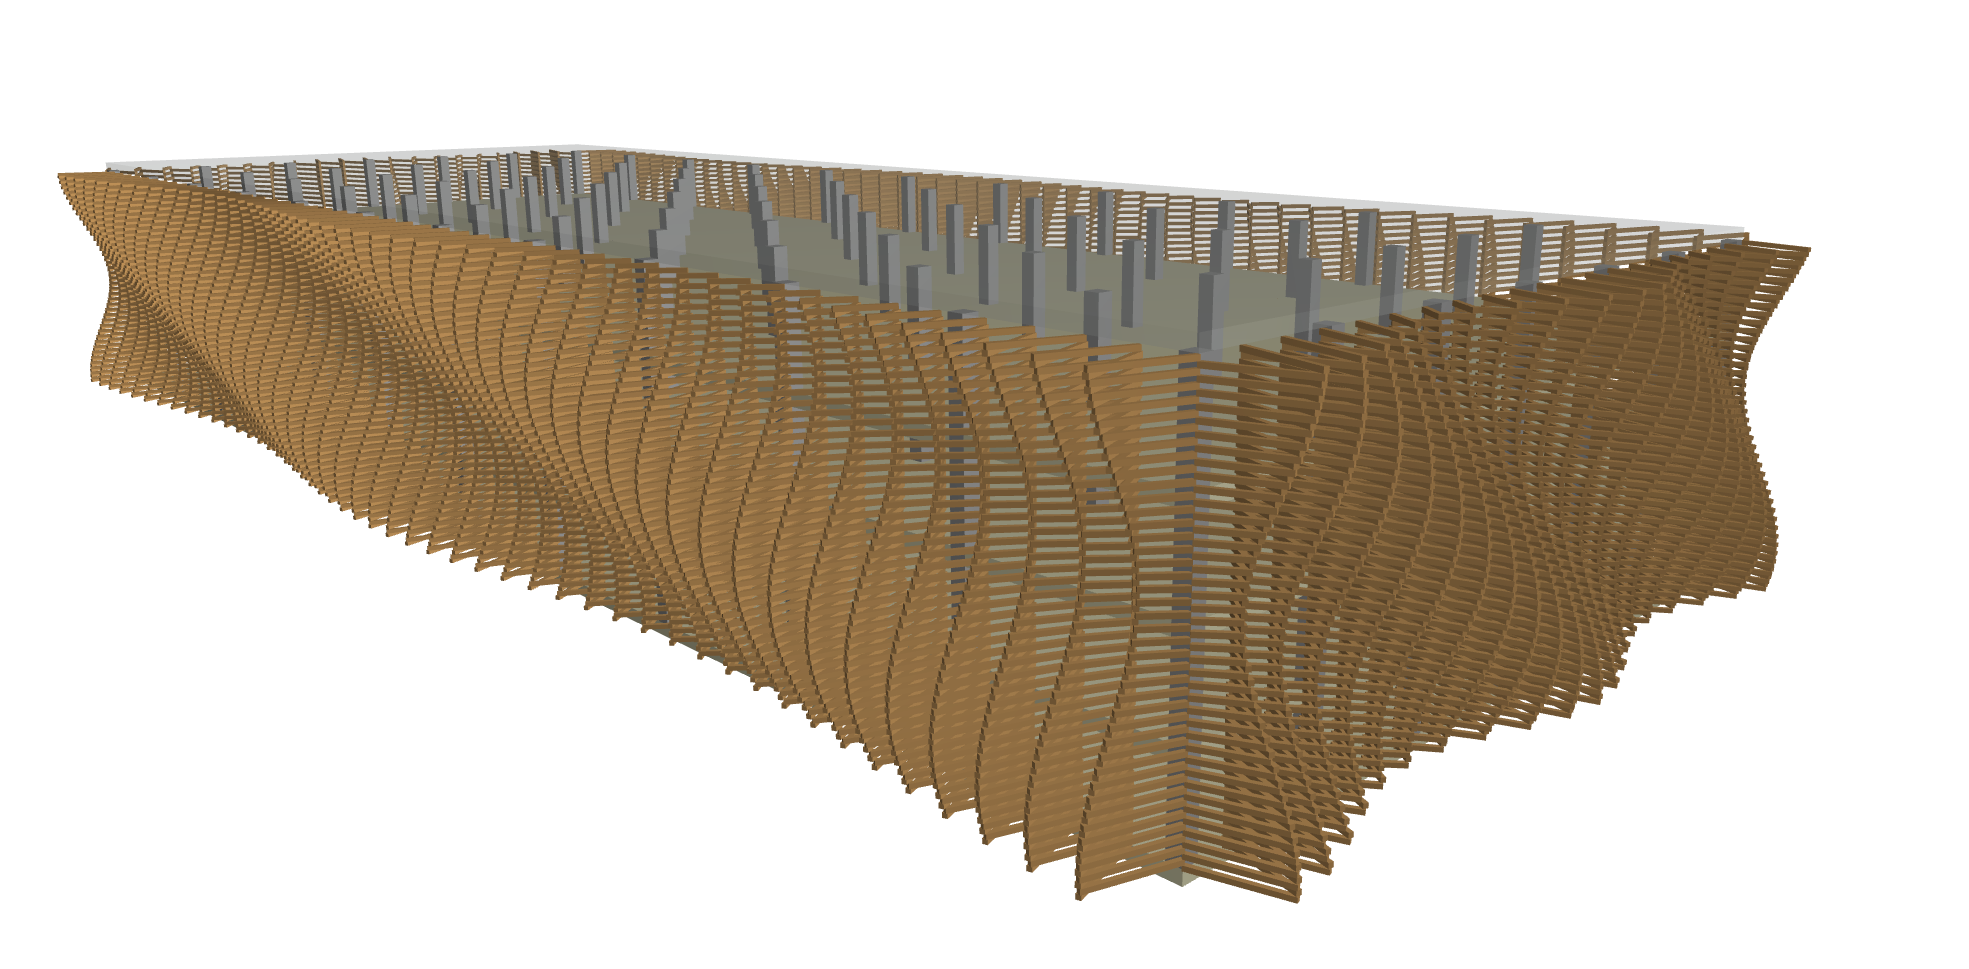
\includegraphics[width=0.8\textwidth]{images/carmo_render}
	\caption{Rendering of a building design made using \gls{gd}.}
	\label{fig:carmo:render}
\end{figure}

\begin{figure}
	\centering
	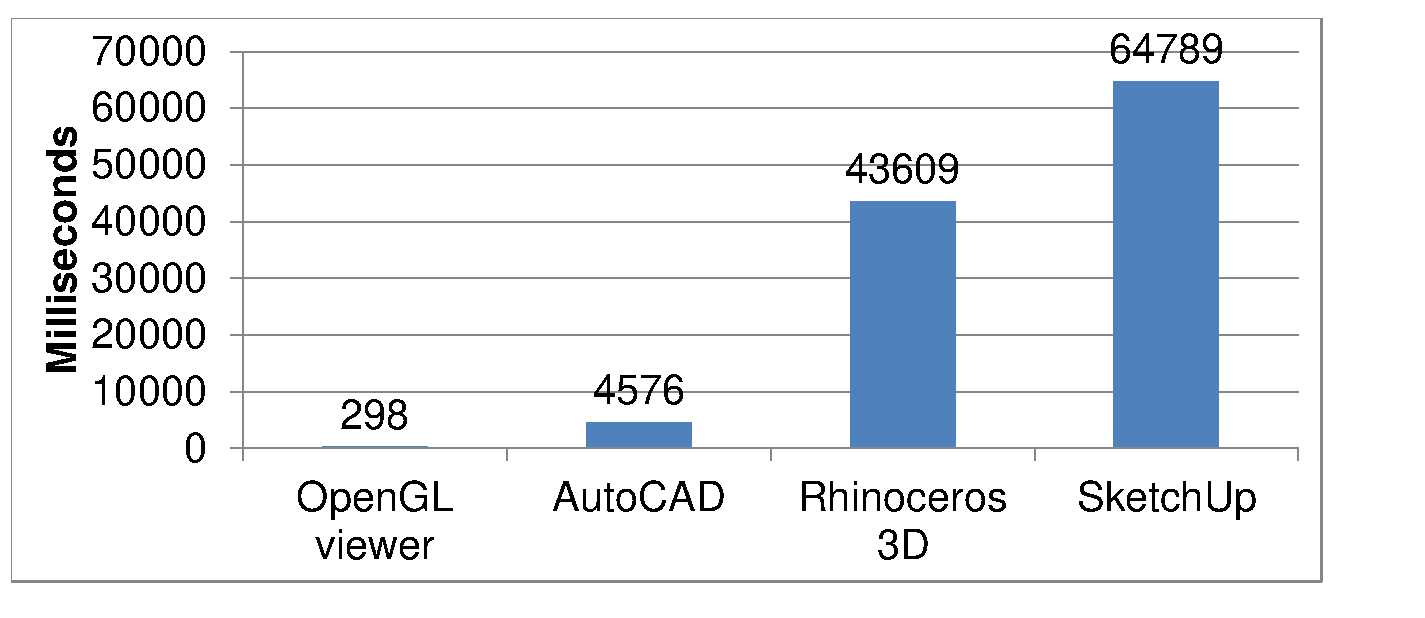
\includegraphics[width=0.8\textwidth]{images/carmo_rosetta_times}
	\caption{Generation times for different \gls{cad} applications using Rosetta.}
	\label{fig:carmo:times}
\end{figure}


\section{Goals}
A \gls{gd} \gls{ide} needs to have more \textbf{accessibility}, not requiring any installation and being available in any computer, and needs to be more \textbf{interactive}, letting architects explore \gls{gd} easily, giving them feedback and showing them the relationship between program and results.
Moreover, it needs to \textbf{integrate} easily with the \gls{cad} applications already used by architects, so they can still integrate their \gls{gd} experiments into their normal workflow.

This thesis aims at increasing architects' productivity when working on \gls{gd} projects by giving them a programming environment in the web specifically for \gls{gd}.
This requires the implementation of a web page that harnesses the performance and graphical capabilities available in modern web browsers, and the implementation of a companion application for allowing models to be exported to traditional \gls{cad} applications.
In this way, architects can write their \gls{gd} programs and visualize the results without being chained to a particular computer, and can easily integrate results into their normal workflow by using the companion application.


\section{Document Structure}
The remainder of this document is structured as follows:
\begin{description}
  \item[Chapter \ref{chapter:background}] explores related work regarding domain-specific \glspl{ide}, with emphasis on those for 3D modeling. A comparison is also presented to show their differences and similarities.
  \item[Chapter \ref{chapter:solution}] presents the details of the solution, its components and how they relate to each other. It also explains how the most important features were implemented.
  \item[Chapter \ref{chapter:evaluation}] evaluates the solution according to the models it can produce and to its performance.
  \item[Chapter \ref{chapter:conclusion}] concludes the document, presenting the main aspects of each chapter and presenting some directions to be considered for future work.
\end{description}


%Identify the problem clearly.
%- There is a need for a widely available 3d modeling tool for architects?
%- Current 3d modeling tools limit are limited to a computer?

%Thesis
%- A web application is the natural step to architecture software?
%--- It centralizes the information on the Internet making it more accessible and affordable.
%---

%Motivation (Benefits of solving the problem?)
%Goals (What we really want to achieve.)
%Contributions (What we have done that can be used by others.) (Separate "Chapter"?)
%Thesis Outline



%State the requirements. What is there a need for?
%- Higher performance, compared to standard modeling tools.
%- Fit into the current workflow of the architect.




%Introduce the context of the work (the currently used tools, etc).
%Smoothly introduce the problem/need for a solution.
%Lastly, clearly state the goals of the work.

%% Bruno Ferreira, Rosetta Revit BIM
%Apareceram os CADs, (evitam redesenhar tudo à mão)
%Apareceram os BIMs, (modelo computacional de arquitetura)
%Ambos têm muito trabalho repetido
%O Generative Design, Procedural modeling apareceram
%Procedural modeling normalmente limitado a um CAD
%Apareceu o Rosetta
%Rosetta só suporta CADs
%Revit(BIM) tem API
%Vamos usá-la para dar suporte para o Revit ao Rosetta
%
%% Uma secção quando muda de assunto.

%% Projecto de tese
%Programação cada vez mais adoptada
%É preciso aprender muitos conceitos e processos e ter muita disciplina
%Os IDEs juntam todas as ferramentas num pacote
%Os IDEs para software industrial são demasiado para iniciantes
%Há IDEs, feitos para certos domínios, mais amigáveis para iniciantes
%Os arquitetos começaram a usar programação para fazer o seu trabalho e também podem usufruir dos benefícios dos IDEs
%Por exemplo, eles usam os IDEs imbutidos em CADs, o Grasshopper, o Processing e o Rosetta
%Estes IDEs são todos instalados, limitando os computadores onde se pode trabalhar
%Pode-se passar IDE para aplicação web
%Tem de suportar gráficos 3D
%No problem, já existem muitas aplicações web com 3D graças ao WebGL.
%Objectivo: Fazer IDE para arquitetura como uma aplicação web
